\documentclass[12pt]{article}
\usepackage[spanish]{babel}
\usepackage{geometry}
\geometry{a4paper, margin=1in}
\usepackage{graphicx}
\usepackage{xcolor}
\usepackage{titlesec}
\usepackage{parskip}
\usepackage{multicol}
\usepackage{cite}
\usepackage{float}

\definecolor{highlight}{RGB}{255, 255, 0}

\titleformat{\section}{\normalfont\Large\bfseries}{\thesection}{1em}{}
\titleformat{\subsection}{\normalfont\large\bfseries}{\thesubsection}{1em}{}

\begin{document}

% Logos
\begin{minipage}{0.45\textwidth}
    
\includegraphics[width=0.4\textwidth]{inFiles/Figures/epnLogo.jpg}
\end{minipage}
\hfill
\begin{minipage}{0.45\textwidth}
    \raggedleft
    
\includegraphics[width=0.4\textwidth]{inFiles/Figures/FIS_logo.jpg}
\end{minipage}

\vspace{0.5cm}

% Títulos principales
\begin{center}
    \textbf{ESCUELA POLITÉCNICA NACIONAL}\\[0.2cm]
    \textbf{FACULTAD DE INGENIERÍA DE SISTEMAS}\\[0.2cm]
    \textbf{INGENIERÍA {\textbf{EN COMPUTACIÓN}}}
\end{center}

\vspace{0.5cm}
\hrule
\vspace{0.5cm}

% Datos principales
\noindent\textbf{PERÍODO ACADÉMICO:} 2025-A\\[0.2cm]
\noindent\textbf{ASIGNATURA:} ICCD412 Métodos Numéricos \hfill \textbf{GRUPO:} GR2\\[0.2cm]
\noindent\textbf{TIPO DE INSTRUMENTO:} Práctica 3\\[0.2cm]
\noindent\textbf{FECHA DE ENTREGA LÍMITE:} 04/05/2025\\[0.2cm]
\noindent\textbf{ALUMNO:} Murillo Tobar Juan

\vspace{0.5cm}
\hrule
\vspace{1cm}


% Secciones
\section*{TEMA}
Método de la bisección

\vspace{0.5cm}

\section*{OBJETIVOS}
\begin{itemize}
    \item Comprender la utilidad del método de bisección para la búsqueda de ceros(soluciones) dentro de un intervalo en donde la función es continua.
    \item Practicar mediante la resolución de ejercicios aplicados el método de bisección.
\end{itemize}

\vspace{0.5cm}

\section*{MARCO TEÓRICO}

\large\textbf{Confinamiento de una raíz}
\normalsize\newline\newline
Dentro del método de bisección, uno de los pasos importantes es el confinamiento de la raíz. Como se menciona en \cite{sauer2013}, el confinamiento se encarga de encontrar un intervalo [a, b] que cumpla con un teorema del valor intermedio.
Dicho teorema se resume a que si se tiene una funcion f que es continua en el intervalo [a, b]  y que satisface $f(a)(b)<0$. Entonces existe una raíz r dentro de dicho intervalo.
\vspace{0.5cm}

\section*{DESARROLLO}
\large\textbf{EJERCICIOS APLICADOS}
\normalsize
\begin{figure}[H]
    \centering
    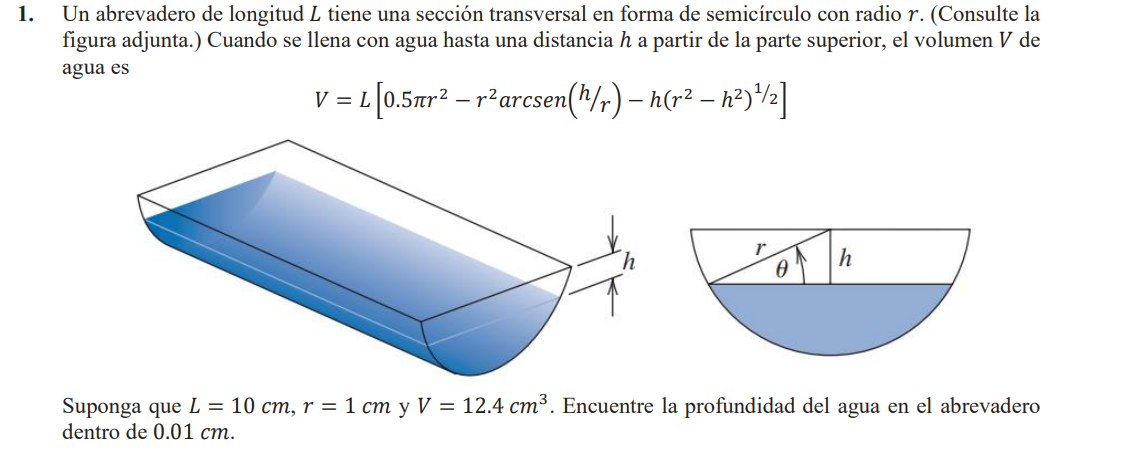
\includegraphics[width=1\textwidth]{./inFiles/Figures/Cap1.png}
    \end{figure}
Primero obtenemos la función $ f = 5\pi-10\arcsen(x)-10x\sqrt{1-x^2}-12.4$.

Ademas este problema confinamos el intervalo a [0, 1] porque el radio es de 1cm y la tolerancia es de $10^{-2}$


\begin{center}
    \begin{tabular}{|c|c|c|c|c|c|c|}
        \hline
        a & b&p&$f(a)$&$f(b)$&$f(p)$&$E_{est}$\\
        \hline
        0& 1   &  0.5    & $3.30796$ & $-12.4$    & $-6.25815$& $0.5$\\
        0& 0.5 &  0.25   & $3.30796$ & $-6.25815$ & $-1.63945$& $0.25$\\
        0& 0.25&  0.125  & $3.30796$ & $-1.63945$ & $0.814489$& $0.125$\\
    0.125& 0.25&  0.1875  & $0.814489$& $-1.63945$& $-0.419947$& $0.0625$\\
    0.125& 0.1875&  0.15625 & $0.814489$& $-0.419947$& $0.195726$& $0.03125$\\
  0.15625& 0.1875& 0.171875 & $0.195726$& $-0.419947$& $-0.112536$& $0.015625$\\
        \hline
      \end{tabular} 
\end{center}

Por lo tanto la profundidad estaría dada por $h \approx 0.171875$ cm.


\begin{figure}[H]
    \centering
    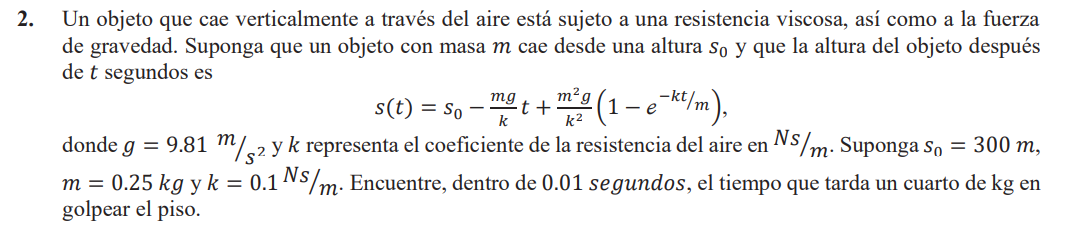
\includegraphics[width=1\textwidth]{./inFiles/Figures/Cap2.png}
\end{figure}


Para empezar a delimitar sabemos que el tiempo empieza desde 0, asi que evaluamos valores al azar hasta obtener uno positivo y uno negativo.
la función $f = 300-\frac{981}{40}x+\frac{981}{16}(1-e^{\frac{-2}{5}x})-0$.

Al final s(t) es 0 porque debe llegar al suelo, y el intervalo será entre [14, 15]
\begin{center}
    \begin{tabular}{|c|c|c|c|c|c|c|}
        \hline
        a & b&p&$f(a)$&$f(b)$&$f(p)$&$E_{est}$\\
        \hline
        14   & 15    &  14.5    & $17.7358$ & $-6.71448$ & $5.51437$& $0.5$\\
        14.5 & 15    &  14.75   & $5.51437$ & $-6.25815$ & $-0.599212$& $0.25$\\
        14.5 & 14.75 &  14.625  & $5.51437$ & $-0.599212$& $2.45780$& $0.125$\\
       14.625& 14.75 &  14.6875 & $2.45780$& $-0.599212$& $0.929348$& $0.0625$\\
     14.6875 & 14.75 & 14.7188 & $0.929348$& $-0.599212$& $0.163858$& $0.03125$\\
     14.7188 & 14.75 & 14.7344 & $0.163858$& $-0.599212$& $-0.217674$& $0.0156$\\
        \hline
      \end{tabular} 
\end{center}
Por lo tanto el tiempo cuando llegue al suelo estaría dado por $t \approx 14.7344$ s.

\begin{figure}[H]
    \centering
    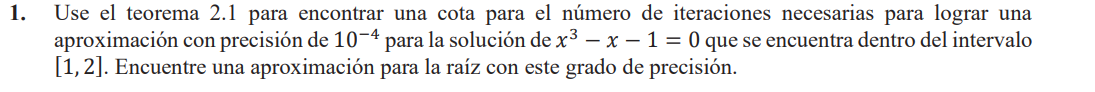
\includegraphics[width=1\textwidth]{./inFiles/Figures/Cap3.png}
\end{figure}

Como sabemos que $\frac{b-a}{2^n} < 10^{-4}$ entonces deducimos que:
$$\frac{1}{2^n} < 10^{-4}$$
$$2^{-n} < 10^{-4}$$
$$\log(2^{-n}) < \log(10^{-4})$$
$$-n\log(2) < -4\times\log(10)$$
$$-n < -4\times\frac{1}{\log(2)}$$
$$ n > \frac{4}{\log(2)}$$

Por lo tanto $n > 13.2877$ o  $n \approx 14$.
\begin{center}
    \begin{tabular}{|c|c|c|c|c|c|c|}
        \hline
        a & b&p&$f(a)$&$f(b)$&$f(p)$&$E_{est}$\\
        \hline
        1       & 2         &  1.5    & $-1$                & $5$                       & $0.875$           & $0.5$\\
        1       & 1.5       &  1.25   & $-1$                & $0.875$                   & $-0.296875$       & $0.25$\\
        1.25    & 1.5       &  1.375  &$-0.296875$          & $0.875$                   & $0.224609$        & $0.125$\\
        1.25    & 1.375     &  1.3125 &$-0.296875$          & $0.224609$                & $-0.0515136$      & $0.0625$\\
        1.3125  & 1.375     &  1.34375& $-0.0515136$        & $0.224609$                & $0.0826111$       & $0.03125$\\
        1.3125  & 1.34375   &  1.32813& $-0.0515136$        & $0.0826111$               & $0.0145974$       & $0.015625$\\
        1.3125  & 1.32813   &  1.32032& $-0.0515136$        & $0.0145974$               & $-0.0186789$      & $7.815*10^{-3}$\\
        1.32032 & 1.32813   &  1.32423& $-0.0186789$        & $0.0145974$               & $-2.08001*10^{-3}$& $3.905*10^{-3}$\\
        1.32423 & 1.32813   &  1.32618& $-2.08001*10^{-3}$  & $0.0145974$               & $6.24357*10^{-3}$ & $1.95*10^{-3}$\\
        1.32423 & 1.32618   &  1.32521& $-2.08001*10^{-3}$  & $6.24357*10^{-3}$         & $2.09934*10^{-3}$ & $9.75*10^{-4}$\\
        1.32423 & 1.32521   &  1.32472& $-2.08001*10^{-3}$  & $2.09934*10^{-3}$         &  $8.71162*10^{-6}$& $4.9*10^{-4}$\\
        1.32423 & 1.32472   &  1.32448& $-2.08001*10^{-3}$  & $8.71162*10^{-6}$         & $-1.01458*10^{-3}$& $2.45*10^{-4}$\\
        1.32448 & 1.32472   &  1.3246& $-1.01458*10^{-3}$  & $8.19138*10^{-4}$         &  $-5.02989*10^{-4}$& $1.2*10^{-4}$\\
        \hline
      \end{tabular} 
\end{center}


La aproximación es 1.3246.
\begin{figure}[H]
    \centering
    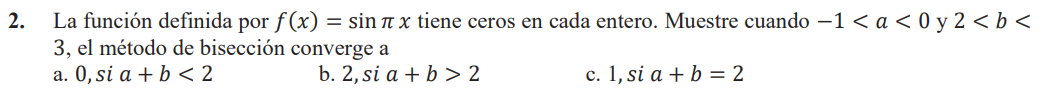
\includegraphics[width=1\textwidth]{./inFiles/Figures/Cap4.png}
\end{figure}

\textbf{a)}
\newline
Tendrías el intervalo (-1, 0) $\cup$(-2, 3). En este caso si convergería porque tenemos varias raíces dentro como el 0.
En este caso debería darse que la parte decimal de a sea mayor a la de b, es decir
$$a < 2-b$$

\textbf{b)}
\newline
Tendrías el intervalo (-1, 0) $\cup$(-2, 3). En este caso si convergería porque tenemos varias raíces dentro como el 2.
En este caso debería darse que la parte decimal de b sea mayor a la de a, es decir
$$a > 2-b$$

\textbf{c)}
\newline
Tomamos un ejemplo como a= -0.5 y b = 2.5, es decir el valor decimal de a debe ser igual al de b para que converja en esta situación.
$$2-b = a$$
\vspace{0.5cm}
\section*{CONCLUSIONES}
\begin{itemize}
    \item El método de bisección nos permite encontrar valores aproximados a incógnitas envueltas en ecuaciones sumamente difíciles de despejar.
    \item Al realizar los ejercicios se logro relacionar problemas de la vida real con el método de bisección.
\end{itemize}
\vspace{0.5cm}
\section*{RECOMENDACIONES}
\begin{itemize}
    \item El confinamiento de la raíz es fundamental para la aplicación del método de bisección. Nos podría ahorrar algunos cálculos.
   
\end{itemize}

\vspace{0.5cm}


\renewcommand{\refname}{\MakeUppercase{REFERENCIAS}}
\bibliographystyle{IEEEtran}
\bibliography{inFiles/References/references.bib}

\end{document}
